% Les versions récentes de xcolor ignorent l'ancienne option `usenames` encore
% transmise par le socle historique kaobook. Masquer uniquement cet avertissement
% avant le chargement de la classe évite de cacher les autres diagnostics.
\RequirePackage{silence}
\WarningFilter{xcolor}{Package option `usenames' is obsolete}

\documentclass[
  fontsize=10pt,
  twoside=true,
]{kaobook}

\usepackage[french]{babel}

% -----------------------------------------------------------------------------
% Mise en page
% -----------------------------------------------------------------------------
\raggedbottom
\setlength{\parindent}{0pt}
\setlength{\emergencystretch}{2em}
\setcounter{topnumber}{5}
\setcounter{bottomnumber}{5}
\setcounter{totalnumber}{8}
\renewcommand{\topfraction}{0.95}
\renewcommand{\bottomfraction}{0.90}
\renewcommand{\textfraction}{0.05}
\renewcommand{\floatpagefraction}{0.80}
\setlength{\floatsep}{8pt plus 2pt minus 2pt}
\setlength{\textfloatsep}{10pt plus 2pt minus 2pt}
\setlength{\intextsep}{8pt plus 2pt minus 2pt}

\newcommand{\discipline}{Sciences Industrielles de l'Ingénieur}
\newcommand{\auteur}{Thomas Lusseau}
\newcommand{\repRel}{../../}
\newcommand{\repStyle}{\repRel/Style}

% Charger en priorité les packages locaux du framework.
\makeatletter
\def\input@path{{../../Style/}}
\makeatother

\input{\repRel/Style/packages_v2}
\input{\repRel/Style/macros_SII_v2}
\input{\repRel/Style/environment_v2}
\pgfplotsset{compat=1.18}

\usepackage{UPSTI_Pedagogique}
\usepackage{CouvertureCours}
\usepackage{TL}
\usepackage{needspace}
\usepackage{etoolbox}
\usepackage{kaotheorems}
\usepackage[normalem]{ulem}

\providecommand{\ul}[1]{\uline{#1}}

\ifdefined\frenchsetup
  \frenchsetup{StandardItemLabels=true}
\fi

\graphicspath{{images/}{./}}
\makeindex[columns=3, title=Index alphabétique, intoc]

\pretocmd{\section}{\Needspace{6\baselineskip}}{}{}
\pretocmd{\subsection}{\Needspace{5\baselineskip}}{}{}
\pretocmd{\subsubsection}{\Needspace{4\baselineskip}}{}{}

\newcommand{\AFfigure}[2][0.96\linewidth]{%
  \begin{center}%
    \IfFileExists{images/#2}{%
      \includegraphics[width=#1]{images/#2}%
    }{%
      \fbox{\parbox[c][35mm][c]{0.88\linewidth}{\centering Illustration à associer}}%
    }%
  \end{center}%
}

% Les hooks anglais de varioref ne sont pas utilisés dans ce cours français.
\makeatletter
\@ifundefined{extrasenglish}{}{\let\extrasenglish\@empty}
\@ifundefined{noextrasenglish}{}{\let\noextrasenglish\@empty}
\makeatother

\begin{document}

\titlehead{Thomas Lusseau - SII en ATS}
\title[Thomas Lusseau - SII en ATS]{Thomas Lusseau - SII en ATS}
\author[TL]{Thomas Lusseau}
\date{\today}

\mainmatter
\setchapterstyle{kao}
\setcounter{margintocdepth}{\sectiontocdepth}
\marginlayout
\pagestyle{scrheadings}

% -----------------------------------------------------------------------------
% Couverture du cours
% -----------------------------------------------------------------------------
\TLCourseCoverSetup
  {images/image3.png}
  {images/image14.png}
  {Cycle 1 : Analyser, expérimenter et\\ communiquer sur les systèmes pluri-\\ technologies}
  {Introduction à l'ingénierie système}
  {\repStyle/png/logo_lycee.png}
  {Lycée Robert Doisneau - ATS}

% Sommaire court : uniquement les sept grandes sections du cours.
\TLCourseCoverContents{%
  \TLCourseContentsLine{1.1}{MISE EN SITUATION}{TL-course-section-1}
  \TLCourseContentsLine{1.2}{Typologie des systèmes}{TL-course-section-2}
  \TLCourseContentsLine{1.3}{L'approche Ingénierie Système}{TL-course-section-3}
  \TLCourseContentsLine{1.4}{Le langage et les diagrammes SysML}{TL-course-section-4}
  \TLCourseContentsLine{1.5}{Architecture fonctionnelle et chaînes fonctionnelles}{TL-course-section-5}
  \TLCourseContentsLine{1.6}{Sources}{TL-course-section-6}
  \TLCourseContentsLine{1.7}{Exercices du chapitre}{TL-course-section-7}
}

\TLCourseFooter
\TLCourseCover
\markboth{Introduction à l'ingénierie système}{Introduction à l'ingénierie système}

\AtBeginEnvironment{corrige}{\small}
\livrettrue
%\livretfalse
\collefalse

% Le fichier historique contenait sa propre couverture et sa propre page de
% chapitre. TLInputCourseBody les retire et commence directement à la section 1.1.
\TLInputCourseBody{01_AnalyseFonctionnelle2022}{images/image3.png}

% Association des illustrations extraites du document Word d'origine.
% Les textes et équations restent composés en LaTeX dans le fichier d'exercices.

\newcommand{\AFoneimage}[2][0.96\linewidth]{%
  \begin{center}\includegraphics[width=#1]{images/#2}\end{center}%
}

\newcommand{\AFtoitDR}{%
\begin{center}
\begin{tikzpicture}[
  x=1cm,y=1cm,
  bloc/.style={draw=bleuxp,fill=bleuxpc,minimum width=2.45cm,
    minimum height=1cm,align=center,font=\bfseries\small},
  rep/.style={draw=gray!70,fill=white,minimum width=2.45cm,
    minimum height=.65cm,align=center,font=\small},
  flux/.style={-Latex,thick,bleuxp}
]
\node[bloc] (alim) at (0,0) {ALIMENTER};
\node[bloc] (dist) at (3,0) {DISTRIBUER};
\node[bloc] (conv) at (6,0) {CONVERTIR};
\node[bloc] (trans) at (9,0) {TRANSMETTRE};
\node[bloc] (agir) at (12,0) {AGIR};
\draw[flux] (alim)--node[above,font=\small]{b : \ldots}(dist);
\draw[flux] (dist)--node[above,font=\small]{c : \ldots}(conv);
\draw[flux] (conv)--node[above,font=\small]{d : \ldots}(trans);
\draw[flux] (trans)--node[above,font=\small]{e : \ldots}(agir);
\node[rep] at (0,-1.25) {A : \ldots};
\node[rep] at (3,-1.25) {B : \ldots};
\node[rep] at (6,-1.25) {C : \ldots};
\node[rep] at (9,-1.25) {D : \ldots};
\node[above,font=\small] at (-1.55,0) {a : \ldots};
\end{tikzpicture}
\end{center}
}

\renewcommand{\AFfigure}[2][0.96\linewidth]{%
\IfStrEqCase{#2}{%
  {af_exo_toit_overview.jpg}{%
    \begin{center}\setlength{\tabcolsep}{2pt}
    \begin{tabular}{ccc}
    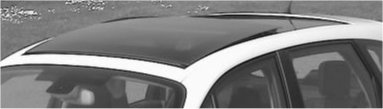
\includegraphics[width=.285\textwidth]{images/image86.jpeg}&
    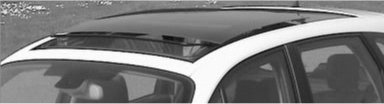
\includegraphics[width=.285\textwidth]{images/image87.jpeg}&
    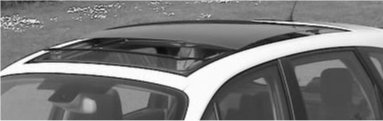
\includegraphics[width=.285\textwidth]{images/image88.jpeg}\\[2mm]
    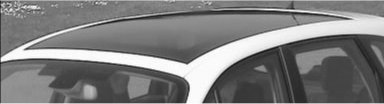
\includegraphics[width=.285\textwidth]{images/image89.jpeg}&
    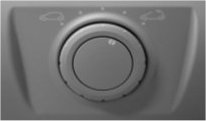
\includegraphics[width=.20\textwidth]{images/image90.jpeg}&
    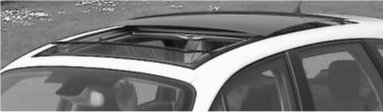
\includegraphics[width=.285\textwidth]{images/image91.jpeg}
    \end{tabular}\end{center}%
  }%
  {af_exo_toit_dr.jpg}{\AFtoitDR}%
  {af_exo_lyre_overview.jpg}{%
    \begin{center}
    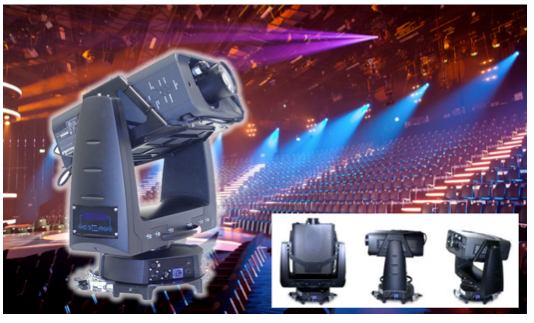
\includegraphics[width=.42\linewidth]{images/image95.png}\hfill
    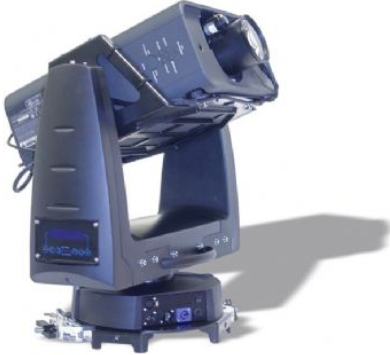
\includegraphics[width=.33\linewidth]{images/image100.png}\par\medskip
    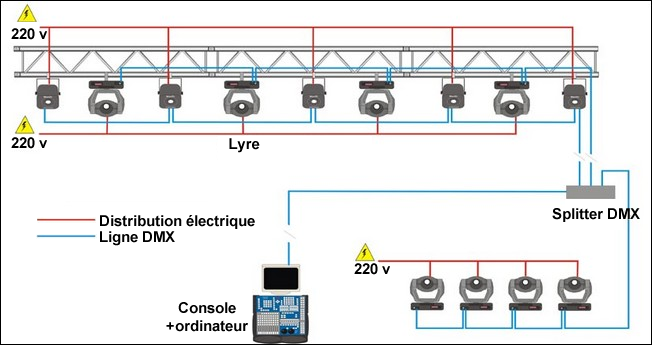
\includegraphics[width=.78\linewidth]{images/image97.png}
    \end{center}%
  }%
  {af_exo_lyre_req.jpg}{\AFoneimage[.85\linewidth]{image98.png}}%
  {af_exo_lyre_bdd.jpg}{\AFoneimage[.92\linewidth]{image99.png}}%
  {af_exo_egreneur_overview.jpg}{%
    \begin{center}
    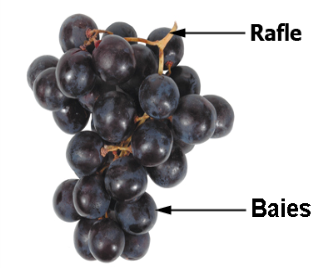
\includegraphics[width=.34\linewidth]{images/image104.png}\hfill
    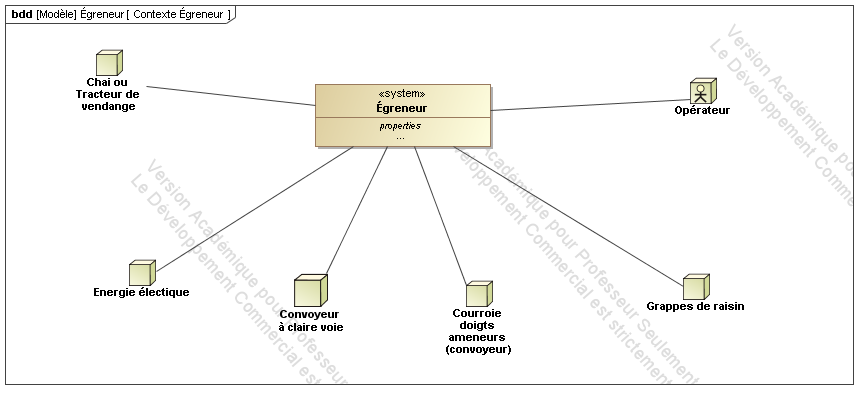
\includegraphics[width=.58\linewidth]{images/image105.png}
    \end{center}%
  }%
  {af_exo_egreneur_bdd.jpg}{\AFoneimage[.87\linewidth]{image106.jpeg}}%
  {af_exo_egreneur_req_ibd.jpg}{%
    \begin{center}
    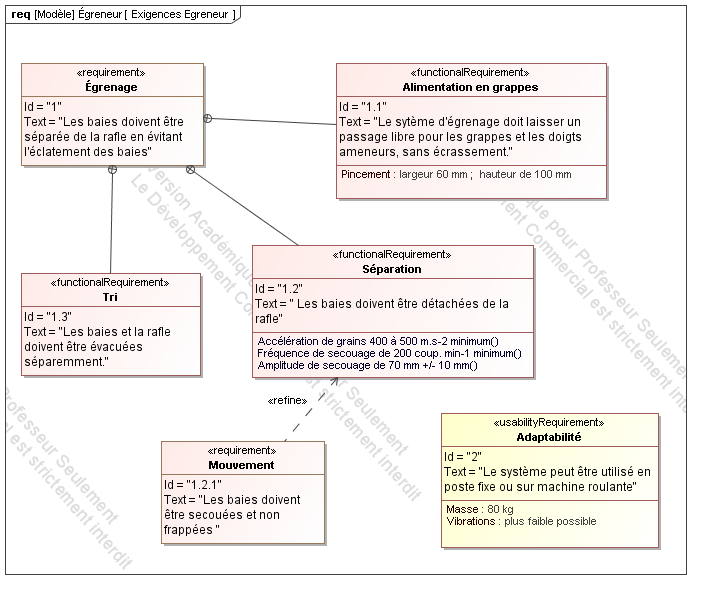
\includegraphics[width=.48\linewidth]{images/image108.png}\hfill
    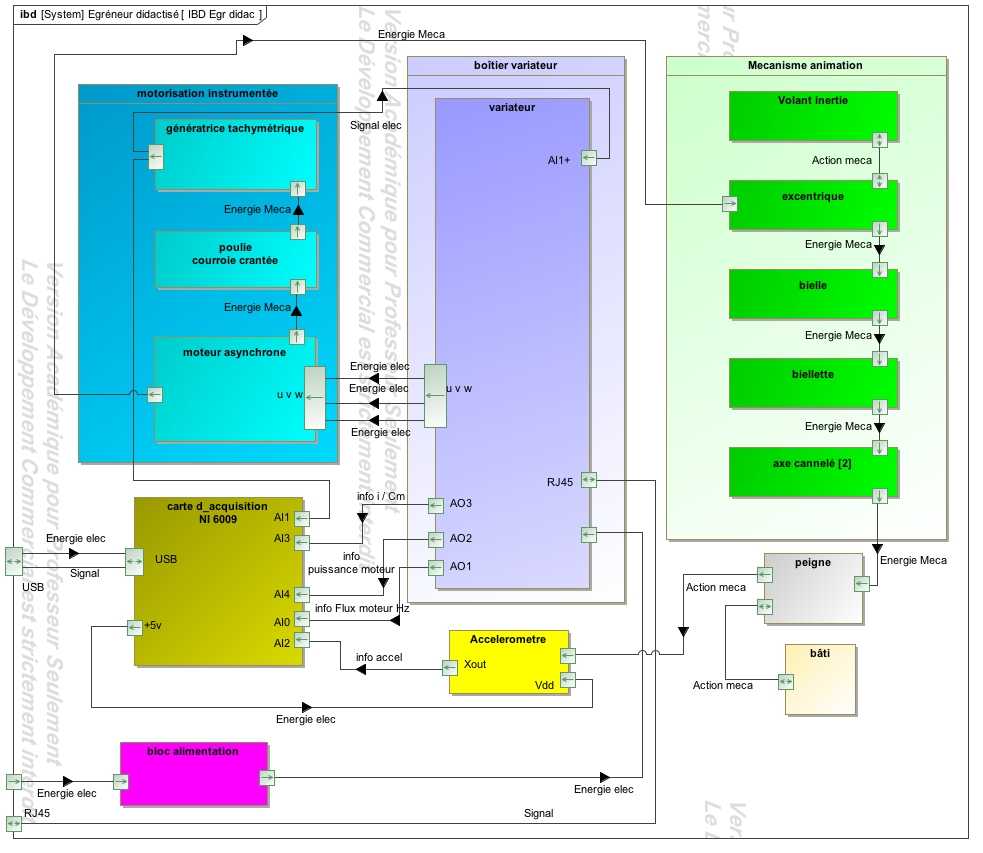
\includegraphics[width=.48\linewidth]{images/image107.jpeg}
    \end{center}%
  }%
  {af_exo_segway_overview.jpg}{\AFoneimage[.55\linewidth]{image109.png}}%
  {af_exo_segway_req.jpg}{\AFoneimage[.90\linewidth]{image111.png}}%
  {af_exo_radiologie_overview.jpg}{\AFoneimage[.78\linewidth]{image112.png}}%
  {af_exo_radiologie_ibd.jpg}{\AFoneimage[.86\linewidth]{image114.png}}%
  {af_exo_secateur_overview.jpg}{%
    \begin{center}
    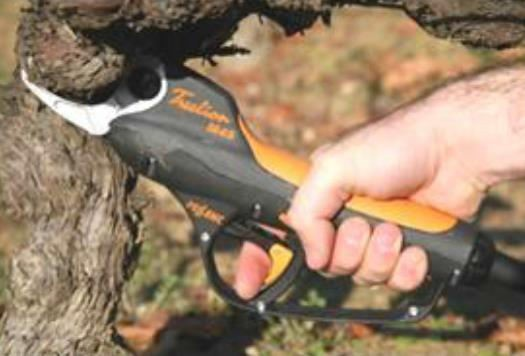
\includegraphics[width=.43\linewidth]{images/image115.jpeg}\hfill
    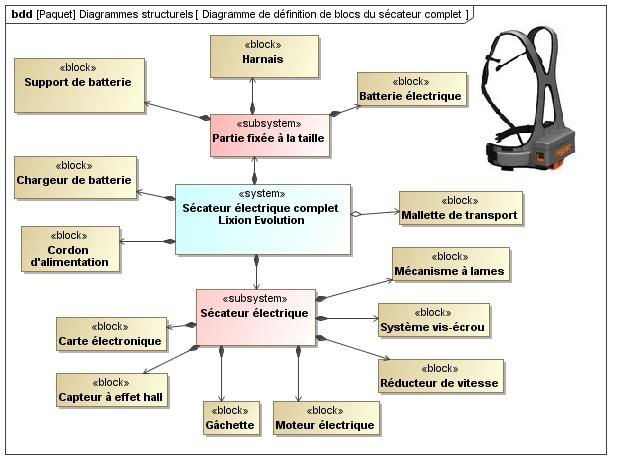
\includegraphics[width=.52\linewidth]{images/image116.jpeg}
    \end{center}%
  }%
  {af_exo_secateur_ibd.jpg}{%
    \begin{center}
    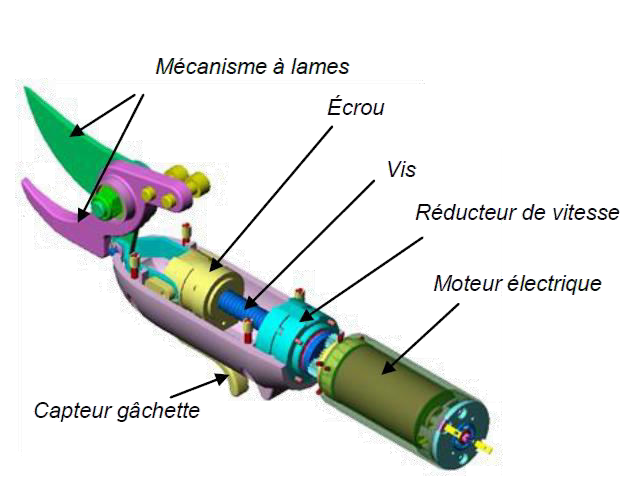
\includegraphics[width=.54\linewidth]{images/image117.png}\hfill
    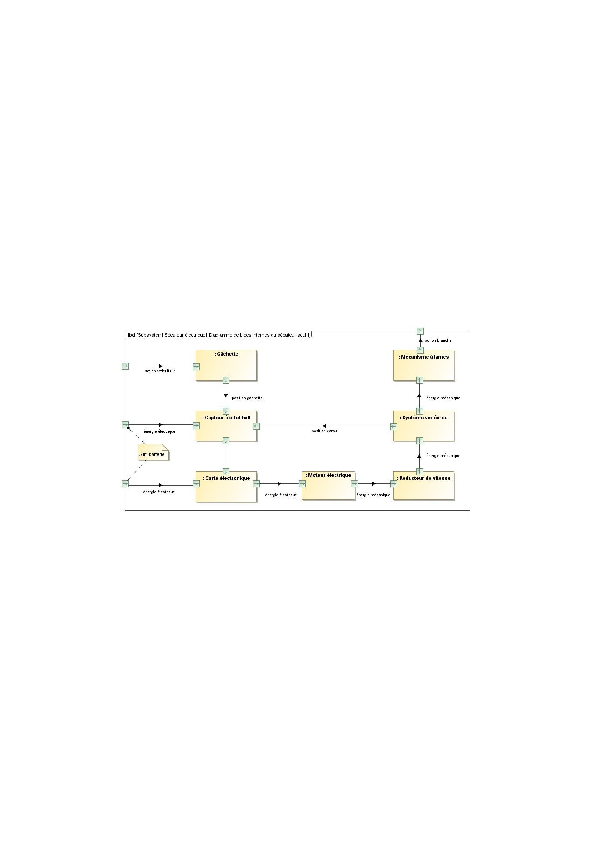
\includegraphics[width=.37\linewidth]{images/image118.png}
    \end{center}%
  }%
  {af_exo_secateur_dr.jpg}{\AFoneimage[.66\linewidth]{image119.png}}%
  {af_exo_prothese_overview.jpg}{%
    \begin{center}
    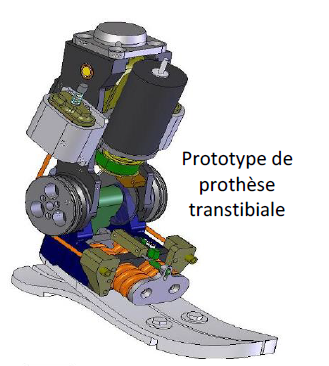
\includegraphics[width=.28\linewidth]{images/image120.png}\hfill
    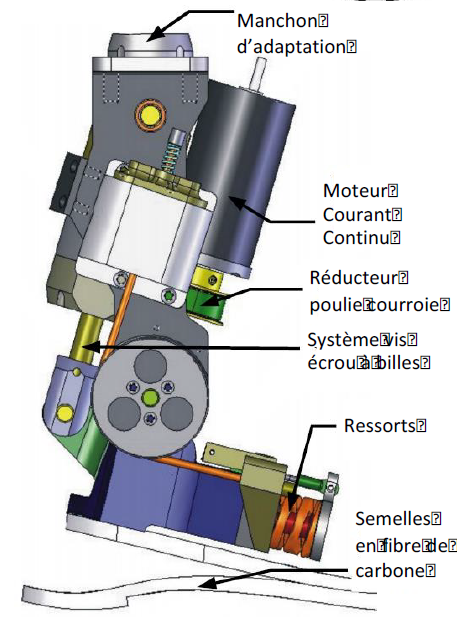
\includegraphics[width=.31\linewidth]{images/image121.png}\hfill
    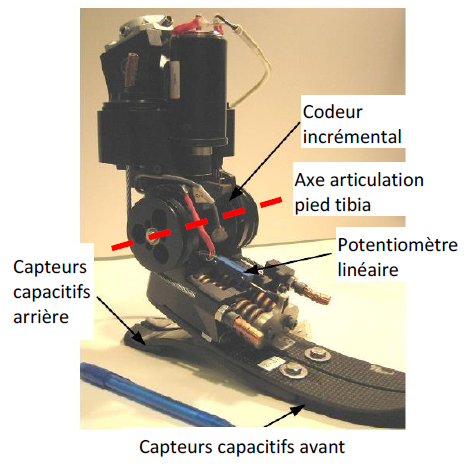
\includegraphics[width=.29\linewidth]{images/image122.png}
    \end{center}%
  }%
  {af_exo_prothese_dr.jpg}{\AFoneimage[.84\linewidth]{image123.png}}%
  {af_exo_tc200_overview.jpg}{%
    \begin{center}
    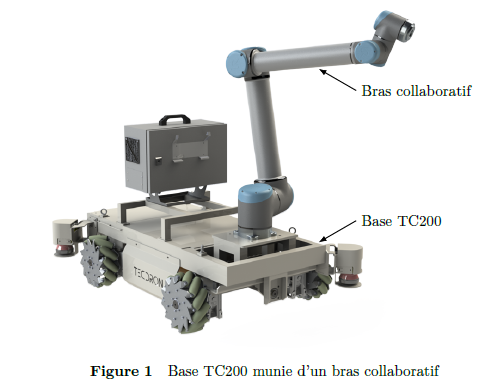
\includegraphics[width=.39\linewidth]{images/image124.png}\hfill
    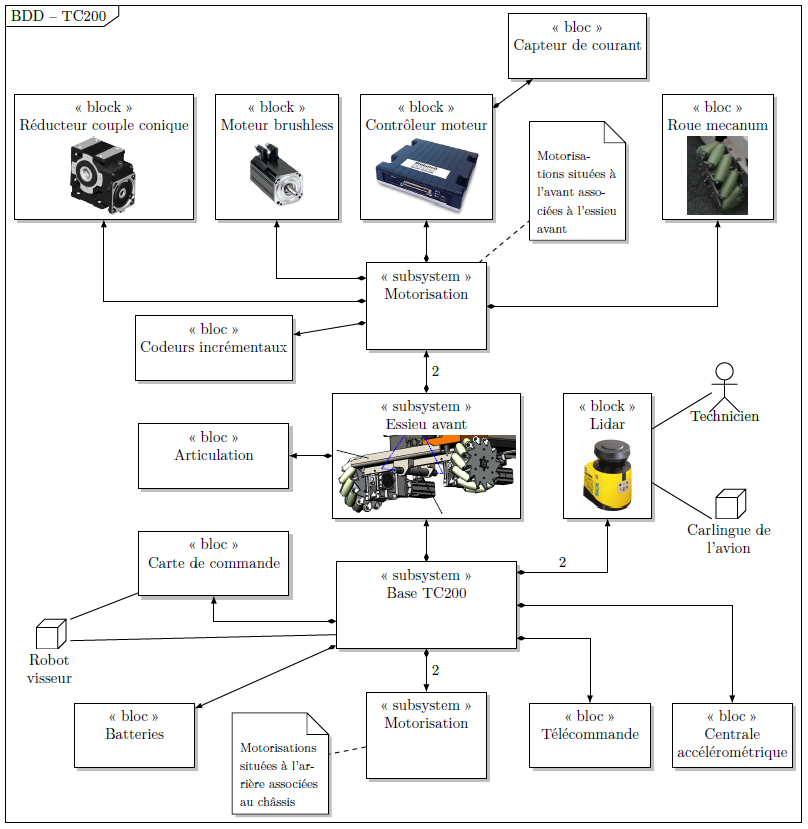
\includegraphics[width=.55\linewidth]{images/image125.png}
    \end{center}%
  }%
  {af_exo_tc200_dr.jpg}{\AFoneimage[.90\linewidth]{image126.png}}%
}[\AFoneimage[#1]{#2}]%
}

% Exercices du chapitre d'analyse fonctionnelle
% Reprise du document de référence 1-AnalyseFonctionnelle.pdf.
% Les textes, questions et équations sont composés en LaTeX ; les diagrammes
% SysML et documents-réponses complexes sont conservés sous forme d'images.

\providecommand{\AFquestion}[2]{%
  \par\medskip\noindent\textbf{Q#1.}~#2\par
}
\providecommand{\AFsource}[1]{%
  \begin{center}\emph{Source : #1}\end{center}
}
\providecommand{\AFfigure}[2][0.96\linewidth]{%
  \begin{center}%
    \IfFileExists{images/#2}{%
      \includegraphics[width=#1]{images/#2}%
    }{%
      \fbox{\parbox[c][35mm][c]{0.88\linewidth}{\centering Illustration absente}}%
    }%
  \end{center}%
}
\providecommand{\AFexotitle}[1]{%
  \clearpage
  \phantomsection
  \addcontentsline{toc}{subsection}{#1}
  \begin{tcolorbox}[
    enhanced,
    colback=white,
    colframe=bleuxp,
    boxrule=0.8pt,
    arc=1mm,
    left=4mm,right=4mm,top=2mm,bottom=2mm,
    fontupper=\bfseries\Large,
    halign=center
  ]
    #1
  \end{tcolorbox}
}
\newtcolorbox{AFexerciseinfo}[1]{
  enhanced,
  breakable,
  colback=bleuxpc,
  colframe=bleuxp,
  boxrule=0.7pt,
  arc=1mm,
  title=#1,
  colbacktitle=bleuxp,
  coltitle=white,
  fonttitle=\bfseries,
  left=3mm,right=3mm,top=2mm,bottom=2mm
}

\clearpage
\pagelayout{wide}
\section{Exercices du chapitre}
\label{exercices-du-chapitre}
\label{TL-course-section-7}

\begin{center}
  
\includegraphics[width=0.42\linewidth]{images/image52.png}
\end{center}

% -----------------------------------------------------------------------------
\AFexotitle{Étude d'un toit ouvrant}
\AFsource{E3A PSI 2006}

\subsubsection*{Mise en situation}

Le toit ouvrant est un sous-système du véhicule automobile qui permet une
meilleure ventilation de l'habitacle et procure aux passagers des sensations de
liberté et une meilleure luminosité. Il s'intègre parfaitement dans les nouveaux
concepts d'adaptation de l'environnement du véhicule aux besoins du conducteur
et des passagers. Les fabricants proposent des gammes de produits qui se
déclinent majoritairement en modèles à énergie électrique, intégrant des
possibilités de commande de plus en plus sophistiquées.

Le modèle étudié se compose d'une glace de sécurité teintée et appartient à la
classe des toits coulissants. Sa cinématique d'ouverture permet un mode
entrebâillant. Il existe en deux modèles : le modèle Medium
($782\times412~\mathrm{mm}$, avec une ouverture entrebâillée de
$43~\mathrm{mm}$) et le modèle Large ($842\times503~\mathrm{mm}$, avec une
ouverture entrebâillée de $48~\mathrm{mm}$). Ils sont équipés d'un déflecteur et
d'un pare-soleil. Le système de commande possède cinq positions stables :

\begin{itemize}
  \item quatre positions de commande : ouvert, entrebâillé, fermé, et impulsionnel ;
  \item une position de repos.
\end{itemize}

\AFimgToitOverview{\linewidth}

\begin{AFexerciseinfo}{Travail demandé}
L'objectif est d'identifier les fonctions assurées par le toit ouvrant et de
compléter les documents fonctionnels proposés.
\end{AFexerciseinfo}

\AFquestion{1}{Préciser la fonction principale du toit ouvrant.}
\AFquestion{2}{Identifier les éléments de l'environnement extérieur qui
interagissent avec le système.}
\AFquestion{3}{Compléter le diagramme d'exigences associé au système.}
\AFquestion{4}{Compléter la chaîne fonctionnelle sur le document-réponse.}

\AFimgToitDR{\linewidth}

% -----------------------------------------------------------------------------
\AFexotitle{Étude d'une lyre instrumentée}

\subsubsection*{Mise en situation}

La lyre instrumentée est destinée à l'étude et à la caractérisation des efforts
appliqués à une structure. Elle associe une partie mécanique, des capteurs et une
chaîne d'acquisition permettant d'exploiter les mesures.

\AFimgLyreOverview{\linewidth}

\AFquestion{1}{Identifier les fonctions de service principales du système.}
\AFquestion{2}{Associer chaque exigence à une fonction technique.}
\AFimgLyreReq{\linewidth}
\AFquestion{3}{Compléter le diagramme de définition de blocs.}
\AFimgLyreBdd{\linewidth}

% -----------------------------------------------------------------------------
\AFexotitle{Étude d'un égreneur}

\subsubsection*{Mise en situation}

L'égreneur automatise la séparation et la distribution de produits dans une
chaîne de production. Son fonctionnement fait intervenir une alimentation en
énergie, une commande et une transmission mécanique.

\AFimgEgreneurOverview{\linewidth}
\AFquestion{1}{Décrire la mission globale du système.}
\AFquestion{2}{Identifier les constituants des chaînes d'énergie et
d'information.}
\AFimgEgreneurBdd{\linewidth}
\AFquestion{3}{Compléter le diagramme des exigences et le diagramme de blocs
internes.}
\AFimgEgreneurReqIbd{\linewidth}

% -----------------------------------------------------------------------------
\AFexotitle{Étude d'un Segway}

\subsubsection*{Mise en situation}

Le Segway est un véhicule électrique auto-équilibré destiné au transport d'une
personne. Son pilotage repose sur la mesure de l'inclinaison du conducteur et sur
la commande coordonnée des deux roues.

\AFimgSegwayOverview{\linewidth}
\AFquestion{1}{Identifier les éléments extérieurs en interaction avec le Segway.}
\AFquestion{2}{Préciser les exigences principales relatives à la sécurité et à
la mobilité.}
\AFimgSegwayReq{\linewidth}

% -----------------------------------------------------------------------------
\AFexotitle{Étude d'un système de radiologie}

\subsubsection*{Mise en situation}

Le système de radiologie permet de positionner un patient et une source de
rayons X afin de réaliser des acquisitions médicales dans des conditions de
sécurité et de précision imposées.

\AFimgRadiologieOverview{\linewidth}
\AFquestion{1}{Définir la fonction principale du système.}
\AFquestion{2}{Identifier les contraintes associées au patient, à l'opérateur et
à l'environnement médical.}

\pagelayout{margin}


\end{document}
